% !TeX program = lualatex
% !TeX encoding = utf8
% !BIB program = biber

\documentclass{bachelor_report}

% Додаткові пакети вносіть у цей файл
% to avoid annoying VScode warning
\setlength{\footskip}{3.60004pt}

% for {cases} environment
\usepackage{mathtools}

% fancy vector arrows
\usepackage[h]{esvect}

% for using indicator \mathbbm{1}
\usepackage{bbm}

% bibliography settings
\usepackage[bibstyle=gost-numeric,sorting=none]{biblatex}
\addbibresource{Tsybulnyk diploma thesis.bib}
\usepackage[autostyle=false]{csquotes}
\renewcommand{\bibfont}{}

% font settings
\usepackage{fontspec}
\setmainfont{CMU serif}

% for floating environments
\usepackage{float}

% make LaTeX PDF output copy-and-pasteable
\usepackage{cmap}

% improved microtypography
\usepackage{microtype}

% color settings
\usepackage[dvipsnames]{xcolor}

% tikz package for creating graphics
\usepackage{tikz}
\usetikzlibrary{arrows.meta}

% package for plotting data
\usepackage{pgfplots}
\usepackage{pgfplotstable}
\pgfplotsset{compat=1.3}

% package for advanced tables
\usepackage{tabularray}

% package for including code listings
\usepackage{listings}
\DeclareCaptionLabelFormat{listingcap}{\vspace*{1mm}Програма #2}
\captionsetup[lstlisting]{margin=0pt, singlelinecheck=false, labelfont=bf, textfont=normalfont, justification=justified, labelsep=endash, labelformat=listingcap, font={Large, stretch=1.5}}

% code listing settings
\lstset{
    frame = single,
    language = Python,
    aboveskip = 3mm,
    belowskip = 3mm,
    columns = flexible,
    basicstyle = \linespread{1}\small\ttfamily,
    numbers = left,
    numberstyle = \tiny\color{gray},
    commentstyle = \color{OliveGreen},
    % stringstyle = \color{Mahogany},
    morestring = [b]''',
    showstringspaces = false,
    morekeywords = {import, as, for, while, in, return, range},
    keywordstyle = \bfseries\color{blue!50!black},
    emph = {[1]import, as, for, while, in, return},
    emphstyle = {[1]\bfseries\color{magenta!60!black}},
    breaklines = true,
    breakatwhitespace = true,
    tabsize = 4,
}

% set page background color (dark read mode)
% \pagecolor[rgb]{0.118,0.118,0.118}
% \color[rgb]{0.8,0.8,0.8}

% Додаткові визначення та перевизначення команд вносіть у цей файл
%%% У даному файлі визначайте всі необхідні вам нові команди TeX
%%% або робіть перевизначення існуючих, наприклад...

\renewcommand{\theequation}{\thechapter.\arabic{equation}} % Номерація формул всередині секцій
\DeclareMathOperator*{\argmin}{argmin}
\DeclareMathOperator*{\argmax}{argmax}

\newcommand*{\scaleq}[2][4]{\scalebox{#1}{$#2$}}%

\renewcommand{\lstlistingname}{Algorithm} % зміна формату підпису блоків коду

% Відомості про автора роботи
%%% Основные сведения %%%
\newcommand{\reportAuthor}             % ФИО автора
{Цибульник А. В.}
\newcommand{\reportAuthorGroup}        % группа автора
{ФІ-91}
\newcommand{\reportTitle}              % Название (тема исследования)
{Програмна реалізація алгоритмів розв'язування задачі побудови оцінок параметрів частково спостережуваного ланцюга Маркова на бінарних послідовностях}
%% використовуйте символ "\par" або "\\" для розбиття назви на декілька рядків

\newcommand{\supervisorFio}            % Керівник практики
{Пономаренко О. В.}
\newcommand{\supervisorRegalia}        % Керівник практики, регалії
{к.т.н., доцент}

% Починаємо верстку документа
\begin{document}

\setfontsize{14}

% Створюємо титульну сторінку
% Титульный лист
\thispagestyle{empty}

\begin{center}
НАЦІОНАЛЬНИЙ ТЕХНІЧНИЙ УНІВЕРСИТЕТ УКРАЇНИ \par
<<КИЇВСЬКИЙ ПОЛІТЕХНІЧНИЙ ІНСТИТУТ ім. Ігоря СІКОРСЬКОГО>>\par
НАВЧАЛЬНО-НАУКОВИЙ ФІЗИКО-ТЕХНІЧНИЙ ІНСТИТУТ\par
Кафедра математичного моделювання та аналізу даних

\vfill
{\huge Звіт з переддипломної практики \par}
\vspace{5mm}
\large\MakeUppercase{\textbf{\reportTitle}} \par
\end{center}

\vfill
\begin{flushright}
Виконав:

студент групи \reportAuthorGroup

\reportAuthor

\vspace{20mm}
Керівник:

\supervisorRegalia

\supervisorFio

\vspace{20mm}
Захистив з оцінкою:

\end{flushright}

\vspace{20mm}
\begin{center}
{Київ~--- 2023}
\end{center}

\newpage
\thispagestyle{plain}


%% Створюємо зміст    % -- розкоментуйте, якщо зміст вам потрібен
%\pagenumbering{gobble}
\tableofcontents
\cleardoublepage
%\pagenumbering{arabic}

% \setcounter{page}{3}    %!!! -- продумати, як автоматизувати номер сторінки

%% Якщо ви використовуєте зміст, то прослідкуйте, щоб номер сторінки 
%% співпадав із справжнім!

% Створюємо перелік умовних позначень, скорочень і термінів
% Якщо цей розділ вам не потрібен, просто закоментуйте два наступних рядка
% \shortings
% %!TEX root = ../thesis.tex
$\mathbbm{1}$ --- індикаторна функція;

$\mathbbm{N}$ --- множина натуральних чисел;

$\forall$ --- квантор загальності: будь-який або для всiх;

Вип. вел. / в. в. --- випадкова величина;

ЗВЧ --- закон великих чисел;

ПММ --- прихована марковська модель.

% Створюємо вступ
\intro
%!TEX root = ../thesis.tex
% створюємо вступ
Марковські моделі мають широкий та ефективний арсенал інструментів для аналізу динаміки систем, поведінка яких у кожен наступний момент часу зумовлюється лише поточним станом системи та не залежить від характеру еволюції у попередні моменти часу. 

Водночас у випадку, коли безпосереднє спостереження еволюції ланцюга Маркова є неможливим чи обмеженим, застосовують моделі прихованих ланцюгів Маркова (ПММ). У такому випадку аналіз поведінки процесу відбувається за деякою опосередкованою інформацією про <<приховані>>, справжні стани ланцюга. 

Наприклад, в біоінформатиці~\cite[глава 9]{Koski2001} апарат ланцюгів Маркова застосовують при дослідженні еволюції молекул ДНК протягом певного часу, вважаючи при цьому за стан системи зв'язану послідовність так званих нуклеотидів, які формуються над алфавітом чотирьох азотистих основ $\{\text{T, C, A, G} \}$.  

Існування статистичних залежностей в чергуванні фонем чи слів в природних мовах зумовлює ефективність використання прихованих марковських моделей до таких завдань, як створення голосових команди, служб транскрипції та голосових помічників~\cite{Rabiner1989}.

Не винятком стають і задачі розпізнавання мови жестів~\cite{Chaaraoui2013}: наприклад, представляючи жести як послідовності прихованих станів, ПММ можуть розпізнавати динаміку та варіації рухів рук.

Відтак, враховуючи актуальність вивчення еволюції систем, стани яких є послідовностями чи наборами символів певної довжини, у роботі розглядається ланцюг Маркова на множині двійкових послідовностей, динаміка якого відстежується за зміною в часі набору функціоналів від його станів.

% Створюємо індивідуальне завдання
\individual
% !TeX spellcheck = uk_Ua

У даному звіті викладена експериментальна перевірка ефективності використаних методів та алгоритмів для побудови оцінок невідомих параметрів частково спостережуваного ланцюга Маркова на бінарних послідовностях. А саме, продемонстровано результати таких задач:

\begin{enumerate}
    \item задача навчання: за наявними спостереженнями про динаміку набору функціоналів від станів прихованого ланцюга бінарних послідовностей оцінено керуючий параметр системи, використовуючи математичний апарат прихованих марковських моделей;
    \item задача декодування: за наявними спостереженнями та оцінкою керуючого параметра відновлено ланцюг прихованих станів;
    \item задачу локалізації: за відомими значеннями набору функціоналів від деякої невідомої підмножини стану прихованого ланцюга, оцінено потужність та набір елементів цієї підмножини;
    \item задача навчання, окреслена в пункті 1), враховуючи, що наявні спостереження є зашумленими, спотвореними.
\end{enumerate}

Для проведення чисельного експерименту, на основі якого виконуватиметься висновок щодо ефективності побудованих теоретичних оцінок невідомих параметрів, було розроблено відповідне програмне забезпечення.

% Додаємо глави
% Якщо ваша робота містить менше або більше глав - модифікуйте наступні 
% рядки відповідним чином
%!TEX root = ../thesis.tex

\chapter{Побудова теоретичних оцінок}
\label{chap: theory}  %% відмічайте кожен розділ певною міткою -- на неї наприкінці необхідно посилатись

У цьому розділі окреслимо побудову теоретичних оцінок для параметрів частково спостережуваного ланцюга Маркова на двійкових послідовностях. 

%%% --------------------------------------------------------
\section{Моделювання об'єкта дослідження}
%%% -------------------------------------------------------- 

Розглянемо ланцюг Маркова $\left\{ X^t \right\}_{t=\overline{1,T}}$, який приймає значення зі скінченної множини $E=\{0,1\}^N$~--- множини всеможливих бінарних послідовностей довжини $N$.

Динаміка ланцюга відбувається згідно з узагальненою моделлю Еренфестів: в кожен момент часу $t$ навмання обирається число $j$ з множини індексів $\left\{ 1,2,\ldots,N \right\}$ бінарної послідовності $X^t$ та відповідний елемент стану $X^t_j$ залишається незмінним з імовірністю $p$ або змінюється на протилежний бінарний символ з імовірністю $1-p$.

Як наслідок окресленої динаміки, матриця перехідних імовірностей ланцюга матиме вигляд:
\begin{equation*}\label{eq: A transition probabilities}
    A_{xx'}=P\left( X^{t+1}=x'\,|\,X^{t}=x \right) = 
    \begin{cases*}
        p, & $x'=x$ \\
        \dfrac{1-p}{N}, & 
            $\begin{aligned} 
                & x^{'}_j = 1 - x_j \\ 
                & \forall i \neq j : x^{'}_i=x_i \\ 
            \end{aligned}$ \\ 
        0, & інакше
    \end{cases*}
\end{equation*}

Крім того, інваріантний розподіл $\pi=\left( \pi_x \right)_{x \in E}$ заданого ланцюга є рівномірним, тобто $\pi_x = \frac{1}{2^N}$. Вважатимемо, що початковий розподіл збігається з $\pi$.

\newpage
Наступним кроком введемо послідовність випадкових величин $\left\{ Y^t \right\}_{t=\overline{1,T}}$, які формуються таким чином: 
\begin{equation}\label{eq: observations}
    Y^t = \left( Y^t_k \right)_{k=\overline{1,L}} = \Bigl( \phi\left( X^t,I_k \right) \Bigr)_{k=\overline{1,L}},\ t=\overline{1,T},
\end{equation}
де $I=\left\{ I_1,\ldots,I_L \right\}$~--- задані підмножини множини індексів $\left\{ 1,2,\ldots,N \right\}$, а функціонал $\phi$ визначимо так:
\begin{equation}\label{eq: phi function}
    \phi\left( X^t,I_k \right) = \sum_{i \in I_k} X^t_i
\end{equation}

\begin{claim}
    Послідовність $\left\{ \left( X^t,Y^t \right) \right\}_{t=\overline{1,T}}$ утворює приховану марковську модель $\left( \pi,A,B \right)$, де 
    \begin{equation*}\label{eq: B emission probabilities}
        B_{xy}=P\left( Y^t=y\,|\,X^t=x \right) = \prod\limits_{k=1}^{L} \mathbbm{1}\left( y_k=\sum\limits_{i \in I_k} x_i \right),
    \end{equation*}
    і позначено $\mathbbm{1}$~--- індикаторна функція.
\end{claim}

%%% --------------------------------------------------------
\section{Постановка завдання}
%%% --------------------------------------------------------

За спостереженнями~\eqref{eq: observations} прихованої марковської моделі слід знайти розв'язки задач:
\begin{enumerate}
    \item Оцінити невідомий <<параметр мутації>> $p$ елементів бінарних послідовностей прихованого ланцюга Маркова та декодувати послідовність станів прихованого ланцюга;
    \item Вважаючи, що спостерігається деяке додаткове значення функціонала~\eqref{eq: phi function} від прихованих станів ланцюга по невідомій <<множині неявних індексів>> $I_*$, оцінити потужність цієї множини та відтворити набір її елементів;
    \item Вважаючи, що значення введеного функціонала~\eqref{eq: phi function} від прихованих станів ланцюга по множинах $I_1,\ldots,I_L$ спостерігаються так:
    \begin{equation}\label{eq: distorted phi function}
        \phi\left( X^t,I_k \right) = \sum_{i \in I_k} \widetilde{X}^t_i,\ k=\overline{1,L},
    \end{equation}
    де для $i \in I_k$
    \begin{equation}\label{eq: distorted X states}
        \widetilde{X}^t_i =
        \begin{cases*}
            1 - X^t_i, & з імовірністю $q_k$ \\
            X^t_i, & з імовірністю $1 - q_k$ \\
        \end{cases*},
    \end{equation}
    оцінити невідомий параметр моделі $p$ та ймовірності спотворень $q_1,q_2,\ldots,q_L$.
\end{enumerate}

\subsection{Оцінка невідомого параметра моделі}

\subsection*{Алгоритм навчання Баума-Велша}
\label{section: baum-welch algorithm}

Спостерігаючи~\eqref{eq: observations}, скористаємося методом максимальної правдоподібності, шукаючи оцінку невідомого параметра $p$ таким чином:
\begin{equation*}\label{eq: p ML estomation}
    \widehat{\,p\,} = \argmax\limits_{p} \sum_{x \in E^T} L_{p,x,y},
\end{equation*}
де
\begin{gather}
    L_{p,x,y} = P\, \bigl( X=x,\,Y=y\,|\,p \bigr) \label{eq: likelihood function} \\
    X=x \Longleftrightarrow \left( X^1=x^1,\ldots,X^T=x^T \right) \notag \\
    Y=y \Longleftrightarrow \left( Y^1=y^1,\ldots,Y^T=y^T \right) \notag
\end{gather}

Щоправда, для заданої марковської моделі вигляд функції правдоподібності~\eqref{eq: likelihood function} матиме громіздкий та неможливий для безпосереднього диференціювання вигляд. 

Однак, в такому випадку можна застосувати модифікацію ЕМ-алгоритму для дослідження прихованих ланцюгів Маркова~--- ітераційний алгоритм Баума-Велша~\cite[розділ 15]{Koski2001}. 

Задавши деяке наближення $p^{(0)}$ невідомого параметра $p$, покладемо
\begin{equation*}\label{eq: p MQL estomation}
    p^{(n+1)} = \argmax\limits_{p} Q\left( p^{(n)},p \right),
\end{equation*}
де
\begin{equation}\label{eq: quasi-log likelihood function}
    Q\left( p^{(n)},p \right) = \sum_{x \in E^T}L_{p^{(n)},x,y}\cdot\ln L_{p,x,y}
\end{equation}
є так званою функцією квазі-log правдоподібності.

Доведено~\cite[розділ 4]{Koski2001}, що така ітераційна процедура є збіжною і приводить до точки локального максимуму логарифму функції правдоподібності~\eqref{eq: likelihood function}. 

Максимізація функції~\eqref{eq: quasi-log likelihood function} приводить до такої ітераційної формули переоцінки параметра $p:$
\begin{equation}\label{eq: p baum-welch estimation}
    p^{(n+1)} = p^{(n)}\cdot\frac{\sum\limits_{t=1}^{T-1}\sum\limits_{x \in E} \alpha_t(x)\,B_{xy^{t+1}}\,\beta_{t+1}(x)}{\sum\limits_{t=1}^{T-1}\sum\limits_{x \in E} \alpha_t(x)\,\beta_t(x)},
\end{equation}
де 
\begin{align}
    & \alpha_t(x) = P\left( Y^1=y^1,\ldots,Y^t=y^t,\,X^t=x \,|\, p^{(n)} \right) \label{eq: alpha, forward algorithm coefficients} \\
    & \beta_t(x) = P\left( Y^{t+1}=y^{t+1},\ldots,Y^T=y^T \,|\, X^t=x,\, p^{(n)} \right) \label{eq: beta, backward algorithm coefficients}
\end{align}
так звані коефіцієнти прямого та зворотного ходу відповідно~\cite[розділ 5]{Nilsson2005}. 

\subsection*{Алгоритм декодування Вітербі}

Використовуючи оцінене значення параметра $\widehat{\,p\,}$, отримане в результаті застосування алгоритму навчання Баума-Велша, скористаємося алгоритмом декодування Вітербі~\cite[розділ 6]{Nilsson2005} для пошуку такої послідовності прихованих станів $\widehat{X}^1,\widehat{X}^2,\ldots,\widehat{X}^T$, яка найкращим чином описує наявні спостереження:
\begin{equation*}\label{eq: decoded stated}
    \widehat{X} = \argmax\limits_{x \in E^T} P\left( X=x\,|\,Y=y,\widehat{\,p\,} \right)
\end{equation*}

\subsection{Оцінка множини неявних індексів}

Нехай окрім набору спостережень~\eqref{eq: observations} протягом еволюції ланцюга на кожному кроці $t$ спостерігається деяке додаткове значення $Y^t_{I_*}$ функціонала~\eqref{eq: phi function} від прихованого стану ланцюга по деякій невідомій підмножині індексів $I_* \subseteq \left\{ 1,2,\ldots,N \right\}:$
\begin{equation*}
    Y_{I_*} = \left( Y^t_{I_*} \right)_{t=\overline{1,T}} = \left( \sum_{i \in I_*} X^t_i \right)_{t=\overline{1,T}} 
\end{equation*}

Перш за все, оцінимо потужність множини $I_*$. Зауважимо, що в силу заданого способу еволюції прихованого ланцюга Маркова
\begin{equation*}
    P\left( Y^t_{I_*}=Y^{t+1}_{I_*} \right)=\frac{\left| I_* \right|}{N}\cdot p + \frac{N-\left| I_* \right|}{N}
\end{equation*}

Ця рівність дозволяє побудувати незміщену та змістовну оцінку для потужності $|I_*|$.

\begin{claim}
    Змістовною і незміщеною оцінкою потужності множини $I_*$ є статистика
    \begin{equation}\label{eq: ||I*|| estimation}
        \widehat{|I_*|} = \frac{N}{1-p} \left( 1-\frac{1}{T-1}\sum_{t=1}^{T-1}\mathbbm{1}\left( Y^t_{I_*}=Y^{t+1}_{I_*} \right) \right) 
    \end{equation}
\end{claim}

Аналогічним чином побудуємо оцінку для потужності перетину множини $I_*$ з індексами множин, які задають спостереження моделі. Вказана оцінка дозволить виявити взаємне розташування елементів множини неявних індексів та множини доступних для дослідження елементів прихованого стану ланцюга Маркова.

\newpage
\begin{claim}
    Нехай $H \subseteq I_1 \cup I_2 \cup \ldots \cup I_L$~--- довільна підмножина множини спостережуваних індексів $I_1 \cup I_2 \cup \ldots \cup I_L$. Тоді змістовною та незміщеною оцінкою потужності множини $I_* \cap H$ є статистика
    \begin{equation}\label{eq: ||I* cup H|| estimation}
        \widehat{\,|I_* \cap H|\,} = \tfrac{N}{(T-1)(1-p)} \cdot \sum_{t=1}^{T-1}\mathbbm{1} \left( Y^t_{I_*} \neq Y^{t+1}_{I_*},\, Y^t_H \neq Y^{t+1}_H \right)
    \end{equation}
\end{claim}

Стратегія визначення елементів, які безпосередньо входять в множину $I_*$, складатиметься з декількох кроків:
\begin{enumerate}
    \item із загальної множини індексів $\left\{ 1,2,\ldots,N \right\}$ сформувати всеможливі підмножини довжиною $\widehat{|I_*|}$, тобто вибірку 
    \begin{equation}\label{eq: candidates for I^}
        \left\{ \mathtt{I_1},\mathtt{I_2},\ldots,\mathtt{I}_{C^{\widehat{|I_*|}}_N} \right\}
    \end{equation}
    \item для кожного <<кандидата>> $\mathtt{I_k}$ з множини \eqref{eq: candidates for I^} згенерувати послідовність значень функціонала~\eqref{eq: phi function} від декодованих прихованих станів по відповідних індексах:
    \begin{equation*}
        \widehat{Y\,}_{\mathtt{I_k}} = \left( \widehat{Y\,}^t_{\mathtt{I_k}} \right)_{t=\overline{1,T}} = \left( \sum_{i \in \mathtt{I_k}} \widehat{X}^t_i \right)_{t=\overline{1,T}}
    \end{equation*}
    \item за допомогою деякої заданої міри $d$ оцінити для кожного $\mathtt{I_k}$ відстань між наборами $\widehat{Y\,}_{\mathtt{I_k}}$ та $Y_{I_*}$;
    \item оцінкою $\widehat{I\,}$ множини $I_*$ стане той <<кандидат>> $\mathtt{I_k}$ з множини \eqref{eq: candidates for I^}, для якого $d$ буде найменшою:
    \begin{equation}\label{eq: I^ estimation}
        \widehat{I\,} = \argmin\limits_{1\leqslant k \leqslant C^{\widehat{|I_*|}}_N}{d\left( \widehat{Y\,}_{\mathtt{I_k}}, Y_{I_*} \right)}
    \end{equation}
\end{enumerate}

Міру близькості $d$ між двома невід'ємними цілочисельними множинами $\widehat{Y\,}_{\mathtt{I_k}}$ та $Y_{I_*}$ однакової довжини визначатимемо або за допомогою середньоквадратичної відстані
\begin{equation}\label{eq: square average distance}
    d_{S}\left( \widehat{Y\,}_{\mathtt{I_k}},Y_{I_*} \right) = \sum_{t=1}^{T}\left( \widehat{Y\,}^t_{\mathtt{I_k}} - Y^t_{I_*} \right)^2,
\end{equation}
або користуючись зваженою відстанню Жаккара~\cite{Chierichetti2010}
\begin{equation}\label{eq: weighted Jaccard distance}
    d_{J}\left( \widehat{Y\,}_{\mathtt{I_k}},Y_{I_*} \right) = 1 - \frac{\sum\limits_{t=1}^{T}\min{\left( \widehat{Y\,}^t_{\mathtt{I_k}},Y^t_{I_*} \right)}}{\sum\limits_{t=1}^{T}\max{\left( \widehat{Y\,}^t_{\mathtt{I_k}},Y^t_{I_*} \right)}}
\end{equation}

\subsection{Оцінка коефіцієнтів спотворення}

Припустимо, що значення функціонала~\eqref{eq: phi function} від прихованих станів ланцюга $\left\{ X^t \right\}_{t=\overline{1,T}}$ по множинам $I_1,\ldots,I_L$ спостерігаються із деякими ймовірностями спотворення $q_1,q_2,\ldots,q_L$ згідно~\eqref{eq: distorted phi function} та~\eqref{eq: distorted X states}.

Оцінимо параметр $p$ та вектор імовірностей спотворень $q=\left( q_1,q_2,\ldots,q_L \right)$, використовуючи ітераційний алгоритм Баума-Велша.

\begin{claim}
    Якщо множини $I_1,\ldots,I_L$ є попарно неперетинними, то утворена послідовність $\left\{ \left( X^t,Y^t \right) \right\}_{t=\overline{1,T}}$ є прихованою марковською моделлю $\left( \pi,A,B^q \right)$, де 
    \begin{equation*}
        B^q_{xy} = P\left( Y^t=y\,|\,X^t=x \right) = \prod\limits_{k=1}^{L} P\left( \xi^k_{01}(x) + \xi^k_{11}(x) = y_k \right),
    \end{equation*}
    і для довільного $k=\overline{1,L}$
    % \begin{align*}
    %     & \xi^k_{01}(x) \sim Bin\left( |I_k| - \sum_{i \in I_k} x_i,\, q_k \right) \\
    %     & \xi^k_{11}(x) \sim Bin\left( \sum_{i \in I_k} x_i,\, 1 - q_k \right)
    % \end{align*}
    \begin{equation*}\scaleq[1]{
        \xi^k_{01}(x) \sim Bin\left( |I_k| - \sum\limits_{i \in I_k} x_i,\, q_k \right),\ \xi^k_{11}(x) \sim Bin\left( \sum\limits_{i \in I_k} x_i,\, 1 - q_k \right)}
    \end{equation*}
    є незалежними випадковими величинами. 
\end{claim}

Виберемо деяке початкове наближення моделі $\left( \pi,A^{(0)},B^{q^{(0)}} \right)$, визначимо коефіцієнти прямого~\eqref{eq: alpha, forward algorithm coefficients} та зворотного~\eqref{eq: beta, backward algorithm coefficients} ходу. Тоді ітераційна формула переоцінки параметра $p$ матиме вид:
\begin{equation}\label{eq: distortion p estimation}
    p^{(n+1)} = p^{(n)}\cdot\frac{\sum\limits_{t=1}^{T-1}\sum\limits_{x \in E} \alpha_t(x)\,B^{q^{(n)}}_{xy^{t+1}}\,\beta_{t+1}(x)}{\sum\limits_{t=1}^{T-1}\sum\limits_{x \in E} \alpha_t(x)\,\beta_t(x)},
\end{equation}
а формула переоцінки компонент вектора $\left( q_k \right)_{k=\overline{1,L}}:$ 
\begin{equation}\label{eq: distortion q estimation}
    q_k^{(n+1)} = q_k^{(n)}\cdot\frac{\sum\limits_{t=1}^{T}\sum\limits_{x \in E}\beta_{t}(x)\sum\limits_{x' \in E} \alpha_{t-1}(x')\,A^{(n)}_{x'x}\sum\limits_{i \in I_k}P^{q^{(n)}}_{x,i}}{|I_k|\sum\limits_{t=1}^{T}\sum\limits_{x \in E} \alpha_t(x)\,\beta_t(x)},
\end{equation}
де при $i \in I_m$
\begin{equation*}
    P^{q}_{x,i} = P\left( \widetilde{\xi^m_{01}}(x) + \widetilde{\xi^m_{11}}(x) = y_m + x_i - 1 \right) \cdot \prod\limits_{\substack{k = \overline{1,L} \\ k \neq m}} P\left( \xi^k_{01}(x) + \xi^k_{11}(x) = y_k \right)
\end{equation*}
та
% \begin{align*}
%     & \widetilde{\xi^m_{01}}(x) \sim Bin\left( |I_m| - 1 - \sum_{j \in I_m\setminus\{i\}} x_j,\, q_m \right) \\
%     & \widetilde{\xi^m_{11}}(x) \sim Bin\left(\sum_{j \in I_m\setminus\{i\}} x_j,\, 1 - q_m \right)
% \end{align*}
\begin{equation*}
    \widetilde{\xi^m_{01}}(x) \sim Bin\left( |I_m| - 1 - \sum\limits_{j \in I_m\setminus\{i\}} x_j,\, q_m \right),\ 
    \widetilde{\xi^m_{11}}(x) \sim Bin\left(\sum\limits_{j \in I_m\setminus\{i\}} x_j,\, 1 - q_m \right)
\end{equation*}

Наостанок зауважимо, що при великих значеннях довжини ланцюга $(T>300)$ виникає потреба у шкалюванні~\cite[розділ 5]{Nilsson2005} коефіцієнтів прямого та зворотного ходу, адже їхні значення стають нерозрізнювано малими для обчислювальних ресурсів. Процедура нормування не вносить змін у вигляд ітераційних формул переоцінки~\eqref{eq: p baum-welch estimation}, \eqref{eq: distortion p estimation} чи \eqref{eq: distortion q estimation}.

\chapconclude{\ref{chap: theory}}

Оскільки задана в рамках дослідження модель відповідає означенню прихованої Марковської моделі, пробудову теоретичних оцінок невідомих параметрів було виконано за допомогою математичного апарату ланцюгів Маркова. Крім того, для задачі локалізації було отримано серію оцінок, використовуючи методи математичної статистики. 

У наступному розділі буде продемонстрована експериментальна перевірка ефективності виведених теоретичних оцінок.
%!TEX root = ../thesis.tex
% створюємо розділ
\chapter{Результати чисельного експерименту}
\label{chap: practice}

Для програмної реалізації реалізація алгоритмів розв’язування задачі побудови оцінок невідомих параметрів моделі було використано засоби мови програмування \texttt{Python} версії \texttt{3.8.10} в інтегрованому середовищі розробки \texttt{Visual Studio Code} версії \texttt{1.78.2}.

Вибір мови програмування зумовлювався широким арсеналом вбудованих програмних пакетів мови \texttt{Python} для роботи з масивами даних та математичними обчисленнями (бібліотеки \texttt{NumPy}, \texttt{itertools}, \texttt{SciPy}, \texttt{random}, \texttt{numda}), а також наявними інструментами для візуалізації даних (пакети \texttt{pandas}, \texttt{matplotlib}). Додаток Б містить тексти ключових програмних блоків коду, необхідних для реалізації чисельного експерименту.

Крім того, для ефективного керування великою кількістю взаємопов'язаних програмних блоків (функцій), а також для більш наочної демонстрації отриманих результатів було розроблено графічний інтерфейс користувача засобами пакету \texttt{PySimpleGUI} мови \texttt{Python}. Додаток А містить опис та приклад роботи розробленого програмного модуля.

\section{Оцінка невідомого параметра моделі}

У рамках чисельного експерименту було згенеровано прихований ланцюг Маркова протягом $T=200$ моментів часу для бінарних послідовностей довжини $N=5$ при заданому параметрі моделі $p=0.2$. Множину спостережуваних індексів було задано таким чином:
\begin{equation}\label{eq: example observed indexes}
    I=\{I_1,I_2\}=\{(2,3),(1,4)\}
\end{equation} 

Рис.~\ref{pic: p baum-welch learning algorithm} демонструє збіжність алгоритму Баума-Велша при оцінці параметра $p$. Червоним кольором позначена початкова ітерація $p^{(0)}=0.55$.

\begin{figure}[H]\centering
    \setfontsize{14pt}
    \begin{tikzpicture}
        \begin{axis}[
            xlabel = Ітерації алгоритму,
            ylabel = Значення параметра $\widehat{\,p\,}$,
            scale only axis,
            ymax = 0.62,
            grid = both,
            grid style = {draw=gray!30},
            minor tick num = 4,
            minor grid style = {draw=gray!10},
        ]
            \addplot[blue!80, mark=*] table {Data/baum-welch learning algorithm.txt};
            \addplot[red, mark=*] table {
                n p
                0 0.55
            };
        \end{axis}
    \end{tikzpicture}
    \caption{Ітерації алгоритму Баума-Велша для оцінки параметра $p$}
    \label{pic: p baum-welch learning algorithm}
\end{figure}

За $n=12$ ітерацій алгоритм досягає точності $\varepsilon=0.0001$ переоцінки оцінюваного параметра. При цьому, отримане значення $\widehat{\,p\,}=0.1959$ відрізняється від свого істинного значення $p=0.2$ на величину $\delta=0.0041$.

\section{Алгоритм декодування прихованих станів}

Наступним кроком, отримавши оцінене значення $\widehat{\,p\,}$, декодуємо ланцюг прихованих станів за допомогою алгоритму Вітербі~\cite[розділ 6]{Nilsson2005}. 

Якість отриманих результатів оцінимо через порівняння в кожен момент часу $t$ істинної прихованої бінарної послідовності $X^t$ та декодованої $\widehat{X^t}$ за допомогою відстані Геммінга:
\begin{equation*}
    d_H\left( X^t,\widehat{X^t} \right) = \sum_{i=1}^{N} \mathbbm{1}\left( X^t_i \neq \widehat{X^t_i} \right)
\end{equation*} 

Таким чином, чим більше символів між справжнім та декодованим станами збігаються, тим меншою буде відповідна відстань Геммінга $d_H$. 

\begin{figure}[H]\centering
    \setfontsize{14pt}
    \begin{tikzpicture}
        \begin{axis}[
            symbolic x coords = {$d_H=0$,$d_H=1$,$d_H=2$,$d_H=3$,$d_H=4$,$d_H=5$},
            x tick label style = {font=\footnotesize},
            scale only axis,
            ymin = 0.0,
            xlabel = Значення відстані Геммінга,
            ylabel = Частка серед усіх станів,
            ymajorgrids = true,
            yminorgrids = true,
            grid style = {draw=gray!30},
            minor tick num = 4,
            minor grid style = {draw=gray!10},
            minor x tick style = {draw=none},
        ]
            \addplot [
                ybar,
                bar width=25pt,
                fill=blue!80,
                opacity=0.7,
            ] coordinates {
                ($d_H=0$,0.17) ($d_H=1$,0.375) ($d_H=2$,0.135) ($d_H=3$,0.25) ($d_H=4$,0.045) ($d_H=5$,0.025)
            };
        \end{axis}
    \end{tikzpicture}
    \caption{Результати алгоритму декодування Вітербі}
    \label{pic: viterbi decoding algorithm}
\end{figure}

З гістограми результатів (Рис.~\ref{pic: viterbi decoding algorithm}) видно, що $17\%$ усього ланцюга декодовано правильно. Наявність близько $40\%$ помилок в одному символі може бути наслідком того, що одного елемента стану немає серед спостережуваних областей ланцюга. Крім того, оцінений параметр $\widehat{\,p\,}$ має похибку $\delta=0.0041$ відносно свого істинного значення, що також впливає на результати задачі декодування.

\section{Оцінка множини неявних індексів}

В ролі множини неявних індексів було обрано набір $I_* = (1,3,5)$. В Табл.~\ref{table: dependence between |I_*| and T} показано збіжність змістовної та незміщеної оцінки~\eqref{eq: ||I*|| estimation} потужності $\widehat{|I_*|}$. Бачимо, що довжини ланцюга $T=200$ недостатньо для отримання точної оцінки. 

\begin{table}[H]\centering
    \setfontsize{14pt}
    \caption{Залежність значення оцінки $\widehat{|I_*|}$ від довжини ланцюга}
    \begin{tblr}{
            hlines,vlines,
            colspec={cccccc},
            % colspec={c|c|c|c|c|c},
            % rowspec={c|c|c},
            row{1-3}={mode=math},
        }
        T               & 200    & 400    & 600    & 800    & 1000    \\
        \widehat{\,p\,} & 0.1959 & 0.1823 & 0.1882 & 0.2099 & 0.2092  \\
        \widehat{|I_*|} & 2      & 2      & 2      & 3      & 3       \\
    \end{tblr}
    \label{table: dependence between |I_*| and T}
\end{table} 

Однак, оскільки обране значення $N$ є невеликим, для оцінки потужності множини неявних індексів в такому випадку можна використати емпіричну оцінку вигляду:
\begin{equation*}
    \widehat{|I_*|}=\max\limits_{1\leqslant t \leqslant T} Y^t_{I_*}
\end{equation*}

Застосуємо отримане значення потужності для виразу~\eqref{eq: I^ estimation}, щоб віднайти елементи, які безпосередньо входять в $I_*:$ квадратична відстань~\eqref{eq: square average distance} вказує на сукупність $\widehat{I\,}_S=(1,2,5)$, а зважена відстань Жаккара~\eqref{eq: weighted Jaccard distance}~--- на сукупність $\widehat{I\,}_J=(1,2,3)$.

Дилему можна вирішити шляхом збільшення $T$ та подальшого використання змістовної оцінки~\eqref{eq: ||I* cup H|| estimation} для визначення взаємного розташування елементів множини неявних індексів відносно спостережуваних індексів~\eqref{eq: example observed indexes}.

\section{Оцінка коефіцієнтів спотворення}

Для кожної із спостережуваних областей~\eqref{eq: example observed indexes} змодельованого ланцюга було обрано такі ймовірності викривлення: $q = (q_1,\,q_2) = (0.05,\,0.1)$. 

Рис.~\ref{pic: p distortion baum-welch learning algorithm} та Рис.~\ref{pic: q distortion baum-welch learning algorithm} демонструють результати переоцінки невідомих параметрів моделі. Червоним кольором позначені значення початкових наближень $p^{(0)}=0.55$ та $q^{(0)}=(0.3,\,0.4)$. 

\begin{figure}[H]\centering
    \setfontsize{14pt}
    \begin{tikzpicture}
        \begin{axis}[
            xlabel = Ітерації алгоритму,
            ylabel = Значення параметра $\widehat{\,p\,}$,
            scale only axis,
            ymax = 0.62,
            ymin = 0.18,
            grid = both,
            grid style = {draw=gray!30},
            minor tick num = 4,
            minor grid style = {draw=gray!10},
        ]
            \addplot[blue!80, mark=*] table[x=n, y=p] {Data/baum-welch distortions learning algorithm.txt};
            \addplot[red, mark=*] table[x=n, y=p] {
                n p
                0 0.55
            };
        \end{axis}
    \end{tikzpicture}
    \caption{Ітерації алгоритму Баума-Велша для оцінки параметра $p$, враховуючи спотворення спостережень}
    \label{pic: p distortion baum-welch learning algorithm}
\end{figure}

\begin{figure}[H]\centering
    \setfontsize{14pt}
    \begin{tikzpicture}
        \begin{axis}[
            xlabel = Значення $\widehat{q\,}_1$,
            ylabel = Значення $\widehat{q\,}_2$,
            scale only axis,
            grid = both,
            grid style = {draw=gray!30},
            minor tick num = 4,
            minor grid style = {draw=gray!10},
            x tick label style={
                /pgf/number format/.cd,
                fixed,
                precision=2
            }
            % legend style={at={(0.05,0.95)}, anchor=north west, cells={anchor=west}, draw=none},
        ]
            \addplot[blue!80, mark=*] table[x=q1, y=q2] {Data/baum-welch distortions learning algorithm.txt};
            \addplot[red, mark=*] table[x=q1, y=q2] {
                n p q1 q2
                0 0.55 0.3 0.4
            };
        \end{axis}
    \end{tikzpicture}
    \caption{Ітерації алгоритму Баума-Велша для оцінки компонент вектора $q$, враховуючи спотворення спостережень}
    \label{pic: q distortion baum-welch learning algorithm}
\end{figure}

\newpage
Для досягнення точності переоцінки $\varepsilon=0.0001$ оцінюваного параметра $p$ у випадку спотворених даних знадобилося $n=53$ ітерацій. При цьому, помітне збільшення похибки: отримане значення $\widehat{\,p\,}=0.2559$ відрізняється від свого істинного значення $p=0.2$ на суттєво вищий показник $\delta=0.0559$. Водночас, точність оцінки коефіцієнтів спостворення $\widehat{q\,} = \left( \widehat{q\,}_1,\,\widehat{q\,}_2 \right) = (0.0454,\,0.1184)$ є високою: $\delta=(\delta_1,\,\delta_2)=(0.0046,\,0.0184)$.

\chapconclude{\ref{chap: practice}}

Результати чисельного експерименту продемонстрували ефективність використаних методів, зокрема збіжність побудованих оцінок до істинних значень параметрів при збільшенні кількості спостережень.

% Створюємо висновки
\conclusions
%!TEX root = ../thesis.tex
% створюємо Висновки до всієї роботи
Загальні висновки до роботи повинні підсумовувати усі ваші досягнення у 
даному напрямку досліджень.

% За кожним пунктом завдань, поставлених у вступі, у висновках повинен 
% міститись звіт про виконання: виконано, не виконано, виконано частково (І 
% чому саме так). Наприклад, якщо першим поставленим завданням у вас іде 
% <<огляд літератури за тематикою досліджень>>, то на початку висновків ви 
% повинні зазначити, що <<у ході даної роботи був проведений аналіз 
% опублікованих джерел за тематикою (...), який показав, що (...)>>. Окрім 
% простої констатації про виконання ви повинні навести, які саме результати 
% ви одержали та проінтерпретувати їх з точки зору поставленої задачі, мети 
% та загальної проблематики.

% В ідеалі загальні висновки повинні збиратись з висновків до кожного 
% розділу, але ідеал недосяжний. :) Однак висновки не повинні містити 
% формул, таблиць та рисунків. Дозволяється (та навіть вітається) 
% використовувати числа (на кшталт <<розроблена методика дозволяє підвищити 
% ефективність пустопорожньої балаканини на $2.71\%$>>).

% Наприкінці висновків необхідно зазначити напрямки подальших досліджень: 
% куди саме, як вам вважається, необхідно прямувати наступним дослідникам у 
% даній тематиці.


% Додаємо бібліографію
% Якщо ви володієте магією bibtex-у, використовуйте її та модифікуйте файл 
% з бібліографією відповідним чином
\printbibliography[title={ПЕРЕЛІК ПОСИЛАНЬ}]
\addcontentsline{toc}{chapter}{Перелік посилань}

% Створюємо додатки (дивись у файли додатків для необхідних пояснень)
% Якщо ви маєте меншу або більшу кількість додатків, модифікуйте наступні 
% рядки відповідним чином
% Якщо ви не маєте додатків, просто закоментуйте наступні рядки
%!TEX root = ../thesis.tex
\append{Графічний інтерфейс користувача}
\label{appendix: A}

Розробка програмного забезпечення охоплювала як імплементацію ітераційних формул переоцінки параметрів моделі, так і розробку графічного інтерфейсу користувача для ефективного керування різними блоками коду. 

Наприклад, на малюнку нижче продемонстровано задання необхідних вхідних даних для генерування відповідного ланцюга Маркова для подальшого розв'язання задачі локалізації.

\begin{figure}[H]\centering
    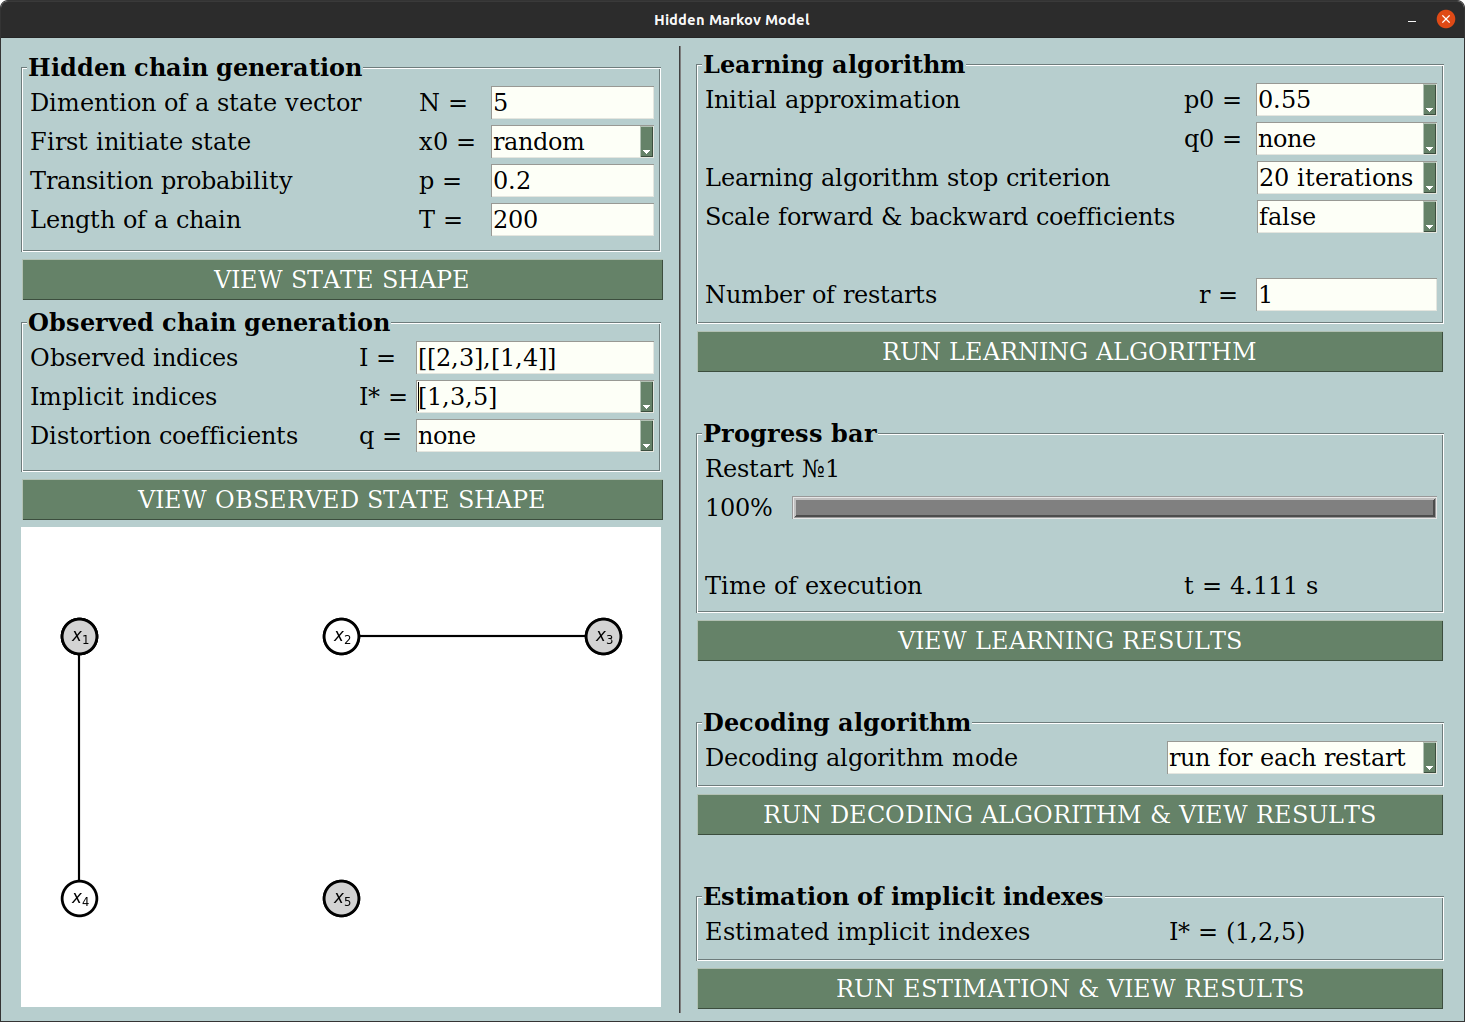
\includegraphics[width=1\linewidth]{Images/GUI.png}
    \caption{Графічний інтерфейс користувача}
    \label{pic: GUI}
\end{figure}

Кожна з відповідних кнопок викликає блоки коду, необхідні для виконання тієї чи іншої задачі. Візуалізація результатів виконується в окремих спливаючих вікнах інтерфейсу у вигляді графіків, наведених у розділі проведення чисельного експерименту.

У лівій нижній частині інтерфейсу схематично зображена конфігурація стану ланцюга: відповідні множини спостережуваних індексів (кожна спостережувана область виокремлюється візуально за з'єднаними ребром вершинами), а також множина неявних індексів, елементи якої позначені сірим кольором.
%!TEX root = ../thesis.tex
\append{Тексти програм}
\label{appendix: B}

У цьому додатку наведені тексти ключових інструментальних програм для проведення експериментальних досліджень. Перелік необхідних бібліотек мови \texttt{Python} наведений нижче:

\vspace{1cm}
\lstinputlisting[linerange={1-7}]{Code/HMM code.py}

\section{Обчислення коефіцієнтів прямого та зворотного ходу}

\lstinputlisting[linerange={9-83}]{Code/HMM code.py}
\vspace{1cm}
\lstinputlisting[linerange={85-140}]{Code/HMM code.py}

\section{Алгоритм Баума-Велша}

\lstinputlisting[linerange={143-255}]{Code/HMM code.py}

\section{Алгоритм Вітербі}

\lstinputlisting[linerange={257-307}]{Code/HMM code.py}

\section{Алгоритм розв'язку задачі локалізації}

\lstinputlisting[linerange={309-389}]{Code/HMM code.py}

% Нарешті
\end{document}